\documentclass[twoside]{book}

% Packages required by doxygen
\usepackage{calc}
\usepackage{doxygen}
\usepackage{graphicx}
\usepackage[utf8]{inputenc}
\usepackage{makeidx}
\usepackage{multicol}
\usepackage{multirow}
\usepackage{textcomp}
\usepackage[table]{xcolor}

% Font selection
\usepackage[T1]{fontenc}
\usepackage{mathptmx}
\usepackage[scaled=.90]{helvet}
\usepackage{courier}
\usepackage{amssymb}
\usepackage{sectsty}
\renewcommand{\familydefault}{\sfdefault}
\allsectionsfont{%
  \fontseries{bc}\selectfont%
  \color{darkgray}%
}
\renewcommand{\DoxyLabelFont}{%
  \fontseries{bc}\selectfont%
  \color{darkgray}%
}

% Page & text layout
\usepackage{geometry}
\geometry{%
  a4paper,%
  top=2.5cm,%
  bottom=2.5cm,%
  left=2.5cm,%
  right=2.5cm%
}
\tolerance=750
\hfuzz=15pt
\hbadness=750
\setlength{\emergencystretch}{15pt}
\setlength{\parindent}{0cm}
\setlength{\parskip}{0.2cm}
\makeatletter
\renewcommand{\paragraph}{%
  \@startsection{paragraph}{4}{0ex}{-1.0ex}{1.0ex}{%
    \normalfont\normalsize\bfseries\SS@parafont%
  }%
}
\renewcommand{\subparagraph}{%
  \@startsection{subparagraph}{5}{0ex}{-1.0ex}{1.0ex}{%
    \normalfont\normalsize\bfseries\SS@subparafont%
  }%
}
\makeatother

% Headers & footers
\usepackage{fancyhdr}
\pagestyle{fancyplain}
\fancyhead[LE]{\fancyplain{}{\bfseries\thepage}}
\fancyhead[CE]{\fancyplain{}{}}
\fancyhead[RE]{\fancyplain{}{\bfseries\leftmark}}
\fancyhead[LO]{\fancyplain{}{\bfseries\rightmark}}
\fancyhead[CO]{\fancyplain{}{}}
\fancyhead[RO]{\fancyplain{}{\bfseries\thepage}}
\fancyfoot[LE]{\fancyplain{}{}}
\fancyfoot[CE]{\fancyplain{}{}}
\fancyfoot[RE]{\fancyplain{}{\bfseries\scriptsize Generated on Thu Apr 2 2015 14\-:18\-:43 for Mirana by Doxygen }}
\fancyfoot[LO]{\fancyplain{}{\bfseries\scriptsize Generated on Thu Apr 2 2015 14\-:18\-:43 for Mirana by Doxygen }}
\fancyfoot[CO]{\fancyplain{}{}}
\fancyfoot[RO]{\fancyplain{}{}}
\renewcommand{\footrulewidth}{0.4pt}
\renewcommand{\chaptermark}[1]{%
  \markboth{#1}{}%
}
\renewcommand{\sectionmark}[1]{%
  \markright{\thesection\ #1}%
}

% Indices & bibliography
\usepackage{natbib}
\usepackage[titles]{tocloft}
\setcounter{tocdepth}{3}
\setcounter{secnumdepth}{5}
\makeindex

% Hyperlinks (required, but should be loaded last)
\usepackage{ifpdf}
\ifpdf
  \usepackage[pdftex,pagebackref=true]{hyperref}
\else
  \usepackage[ps2pdf,pagebackref=true]{hyperref}
\fi
\hypersetup{%
  colorlinks=true,%
  linkcolor=blue,%
  citecolor=blue,%
  unicode%
}

% Custom commands
\newcommand{\clearemptydoublepage}{%
  \newpage{\pagestyle{empty}\cleardoublepage}%
}


%===== C O N T E N T S =====

\begin{document}

% Titlepage & ToC
\hypersetup{pageanchor=false}
\pagenumbering{roman}
\begin{titlepage}
\vspace*{7cm}
\begin{center}%
{\Large Mirana }\\
\vspace*{1cm}
{\large Generated by Doxygen 1.8.6}\\
\vspace*{0.5cm}
{\small Thu Apr 2 2015 14:18:43}\\
\end{center}
\end{titlepage}
\clearemptydoublepage
\tableofcontents
\clearemptydoublepage
\pagenumbering{arabic}
\hypersetup{pageanchor=true}

%--- Begin generated contents ---
\chapter{Mirana}
\label{md_README}
\hypertarget{md_README}{}
A Moving Mesh Toolbox



M\+I\+R\+A\+N\+A stands for \char`\"{}\+Making It Really Adaptive Needs Adapters\char`\"{}. And what this toolbox does is to offer such adapters connecting physical and computational spaces. 
\chapter{Todo List}
\label{todo}
\hypertarget{todo}{}

\begin{DoxyRefList}
\item[\label{todo__todo000001}%
\hypertarget{todo__todo000001}{}%
Module \hyperlink{namespacemirana}{mirana} ]Add mesh derivatives 

add laplacian 
\end{DoxyRefList}
\chapter{Data Type Index}
\section{Data Types List}
Here are the data types with brief descriptions\-:\begin{DoxyCompactList}
\item\contentsline{section}{\hyperlink{classmirana}{mirana} \\*Provide the subroutines \& functions for moving mesh computation }{\pageref{classmirana}}{}
\end{DoxyCompactList}

\chapter{File Index}
\section{File List}
Here is a list of all files with brief descriptions\+:\begin{DoxyCompactList}
\item\contentsline{section}{demo/\hyperlink{example__1_8f90}{example\+\_\+1.\+f90} }{\pageref{example__1_8f90}}{}
\item\contentsline{section}{demo/\hyperlink{example__2_8f90}{example\+\_\+2.\+f90} }{\pageref{example__2_8f90}}{}
\item\contentsline{section}{demo/\hyperlink{example__3_8f90}{example\+\_\+3.\+f90} }{\pageref{example__3_8f90}}{}
\item\contentsline{section}{demo/\hyperlink{example__4_8f90}{example\+\_\+4.\+f90} }{\pageref{example__4_8f90}}{}
\item\contentsline{section}{src/\hyperlink{arms__fgmres_8c}{arms\+\_\+fgmres.\+c} \\*Calling I\+T\+S\+O\+L2 to solve linear equations }{\pageref{arms__fgmres_8c}}{}
\item\contentsline{section}{src/\hyperlink{mirana_8f90}{mirana.\+f90} }{\pageref{mirana_8f90}}{}
\end{DoxyCompactList}

\chapter{Data Type Documentation}
\hypertarget{classmirana}{\section{mirana Module Reference}
\label{classmirana}\index{mirana@{mirana}}
}


Provide the subroutines \& functions for moving mesh computation.  


\subsection*{Public Member Functions}
\begin{DoxyCompactItemize}
\item 
subroutine \hyperlink{classmirana_ab002a22665f70b4c65bdcf70ac96d768}{mirana\-\_\-exception} (message)
\begin{DoxyCompactList}\small\item\em Handling exceptions. \end{DoxyCompactList}\item 
subroutine \hyperlink{classmirana_acccf612b21e3e65bd3a78131c48afe2b}{mirana\-\_\-memory} (name, dim1, dim2)
\begin{DoxyCompactList}\small\item\em Allocate memory for new arrays. \end{DoxyCompactList}\item 
subroutine \hyperlink{classmirana_a9cbee1a318e5e828590c9ccaa51c8472}{save\-\_\-mesh} (mx, my)
\begin{DoxyCompactList}\small\item\em Write mesh data into .dat file for plot. \end{DoxyCompactList}\item 
subroutine \hyperlink{classmirana_a4009036e8b04ac992641e36d34ab0ed4}{d1} (phi, h, phi\-\_\-x)
\begin{DoxyCompactList}\small\item\em Differentiate with respect to the first dimension using central difference. \end{DoxyCompactList}\item 
subroutine \hyperlink{classmirana_a21348ffe170eafc6fc2a009256b1b6e3}{d2} (phi, h, phi\-\_\-y)
\begin{DoxyCompactList}\small\item\em Differentiate with respect to the second dimension using central difference. \end{DoxyCompactList}\item 
subroutine \hyperlink{classmirana_acc84c99770972f6328e89ac04ac67153}{d1h1} (phi, h, phi\-\_\-1h)
\begin{DoxyCompactList}\small\item\em Compute the derivative along the 1st direction at the 1st kind of half points using central difference. \end{DoxyCompactList}\item 
subroutine \hyperlink{classmirana_a9d6168761271912ebfea872e9f322cdc}{d1h2} (phi, h, phi\-\_\-1h)
\begin{DoxyCompactList}\small\item\em Compute the derivative along the 1st direction at the 2nd kind of half points using central difference. \end{DoxyCompactList}\item 
subroutine \hyperlink{classmirana_a9341f957abd27c5132c557ae873055bd}{d2h1} (phi, h, phi\-\_\-2h)
\begin{DoxyCompactList}\small\item\em Compute the derivative along the 2nd direction at the 1st kind of half points using central difference. \end{DoxyCompactList}\item 
subroutine \hyperlink{classmirana_a4f47c93df57dd51d1414b2514fd1b339}{d2h2} (phi, h, phi\-\_\-2h)
\begin{DoxyCompactList}\small\item\em Compute the derivative along the 2nd direction at the 2nd kind of half points using central difference. \end{DoxyCompactList}\item 
subroutine \hyperlink{classmirana_ab9b1e7b5e38c6a020e05196b452e6d02}{d11} (phi, h, phi\-\_\-xx)
\begin{DoxyCompactList}\small\item\em Compute the second order derivative along the first dimension using central difference. \end{DoxyCompactList}\item 
subroutine \hyperlink{classmirana_ae9ee4058ea2b6238b6b745e4468f6a8e}{d12} (phi, h1, h2, phi\-\_\-xy)
\begin{DoxyCompactList}\small\item\em Comopute the mixed second order derivative using central difference. \end{DoxyCompactList}\item 
subroutine \hyperlink{classmirana_a9161b0947ddd188ac99d9246a1d81aed}{d22} (phi, h, phi\-\_\-yy)
\begin{DoxyCompactList}\small\item\em Compute the second order derivative along the second dimension using central difference. \end{DoxyCompactList}\item 
subroutine \hyperlink{classmirana_a353bce8a93046cd8fd25021634d6503e}{dlp} (phi, h1, h2, phi\-\_\-lp)
\begin{DoxyCompactList}\small\item\em Compute Laplacian using central difference. \end{DoxyCompactList}\item 
subroutine \hyperlink{classmirana_a53c223d4530275ef3fc6a5820f5b0990}{nmd} (mx, my, hxi, het, jcb, xi\-\_\-x, xi\-\_\-y, et\-\_\-x, et\-\_\-y)
\begin{DoxyCompactList}\small\item\em (Non-\/conservative Mesh Differentiation) Compute derivatives of mesh grid with respect to computational space and inverse using non-\/conservative form central difference. \end{DoxyCompactList}\item 
subroutine \hyperlink{classmirana_a6b48fffbaaa6f2256928cd73d8891261}{nmd1} (phi, xix, etx, h1, h2, phi\-\_\-x)
\begin{DoxyCompactList}\small\item\em (Non-\/conservative Mesh D1) Compute $\partial\phi/\partial x$ using mesh variables \end{DoxyCompactList}\item 
subroutine \hyperlink{classmirana_a04bd9101c8bdc2f8b69892bd773f3055}{nmd2} (phi, xiy, ety, h1, h2, phi\-\_\-y)
\begin{DoxyCompactList}\small\item\em (Non-\/conservative Mesh D2) Compute $\partial\phi/\partial y$ using mesh variables \end{DoxyCompactList}\item 
subroutine \hyperlink{classmirana_a503a76ad6fbdf28508f8d71786bed518}{nmdlp} (phi, xix, xiy, etx, ety, alp, bet, h1, h2, phi\-\_\-lp)
\begin{DoxyCompactList}\small\item\em (Non-\/conservative Mesh D\-L\-P) Compute $\Delta\phi$ using mesh variables \end{DoxyCompactList}\item 
subroutine \hyperlink{classmirana_a7530ea2e7b2dfe85f3a088d24de59f1d}{greek} (mx, my, xix, xiy, etx, ety, h1, h2, alp, bet)
\begin{DoxyCompactList}\small\item\em Compute the two coefficients for transformed laplacian $\alpha,\beta$. \end{DoxyCompactList}\item 
subroutine \hyperlink{classmirana_a65a514d206d0e8ae53253938d2aff553}{mbc\-\_\-d} (x1, x2, y1, y2)
\begin{DoxyCompactList}\small\item\em (Mesh Boundary Condition for Derivatives) Set the boundary condition of the moving mesh. \end{DoxyCompactList}\end{DoxyCompactItemize}


\subsection{Detailed Description}
Provide the subroutines \& functions for moving mesh computation. 

\begin{DoxyRefDesc}{Todo}
\item[\hyperlink{todo__todo000001}{Todo}]Adapt grid/ to produce desired matrix 

add Sconstruct to compile everything \end{DoxyRefDesc}


\subsection{Member Function/\-Subroutine Documentation}
\hypertarget{classmirana_a4009036e8b04ac992641e36d34ab0ed4}{\index{mirana@{mirana}!d1@{d1}}
\index{d1@{d1}!mirana@{mirana}}
\subsubsection[{d1}]{\setlength{\rightskip}{0pt plus 5cm}subroutine mirana\-::d1 (
\begin{DoxyParamCaption}
\item[{double precision, dimension(\-:,\-:), intent(in), allocatable}]{phi, }
\item[{double precision, intent(in)}]{h, }
\item[{double precision, dimension(\-:,\-:), intent(inout), allocatable}]{phi\-\_\-x}
\end{DoxyParamCaption}
)}}\label{classmirana_a4009036e8b04ac992641e36d34ab0ed4}


Differentiate with respect to the first dimension using central difference. 


\begin{DoxyParams}{Parameters}
{\em phi} & real N1-\/by-\/\-N2 matrix. \\
\hline
{\em h} & real number, step size. \\
\hline
\end{DoxyParams}
\begin{DoxyReturn}{Returns}
phi\-\_\-x real N1-\/by-\/\-N2 matrix, only points ranged in \mbox{[}2\-:(N1-\/1)\mbox{]}X\mbox{[}1\-:N2\mbox{]} are updated. 
\end{DoxyReturn}


Here is the call graph for this function\-:\nopagebreak
\begin{figure}[H]
\begin{center}
\leavevmode
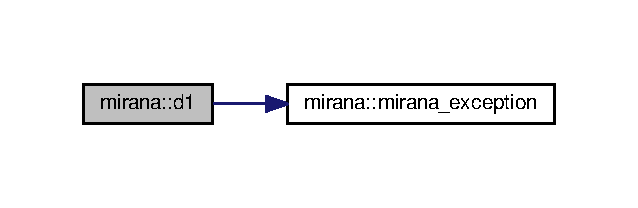
\includegraphics[width=306pt]{classmirana_a4009036e8b04ac992641e36d34ab0ed4_cgraph}
\end{center}
\end{figure}




Here is the caller graph for this function\-:
\nopagebreak
\begin{figure}[H]
\begin{center}
\leavevmode
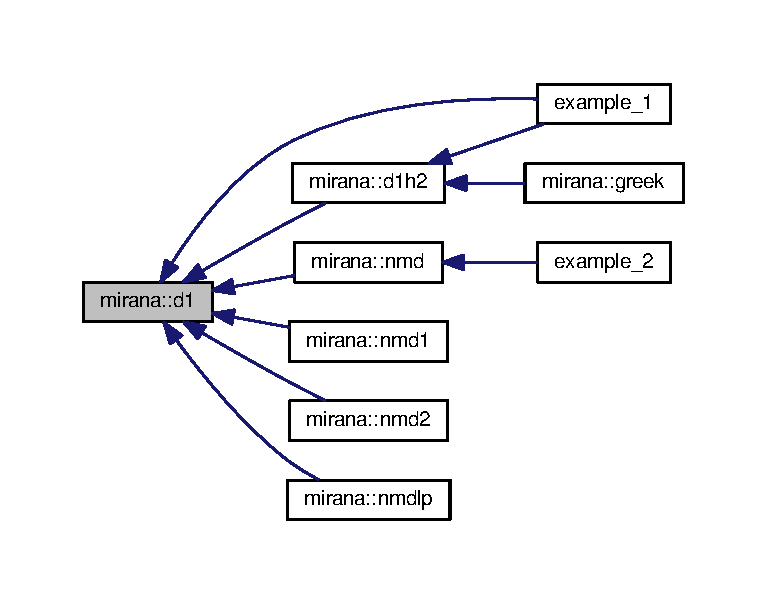
\includegraphics[width=350pt]{classmirana_a4009036e8b04ac992641e36d34ab0ed4_icgraph}
\end{center}
\end{figure}


\hypertarget{classmirana_ab9b1e7b5e38c6a020e05196b452e6d02}{\index{mirana@{mirana}!d11@{d11}}
\index{d11@{d11}!mirana@{mirana}}
\subsubsection[{d11}]{\setlength{\rightskip}{0pt plus 5cm}subroutine mirana\-::d11 (
\begin{DoxyParamCaption}
\item[{double precision, dimension(\-:,\-:), intent(in), allocatable}]{phi, }
\item[{double precision, intent(in)}]{h, }
\item[{double precision, dimension(\-:,\-:), intent(inout), allocatable}]{phi\-\_\-xx}
\end{DoxyParamCaption}
)}}\label{classmirana_ab9b1e7b5e38c6a020e05196b452e6d02}


Compute the second order derivative along the first dimension using central difference. 


\begin{DoxyParams}{Parameters}
{\em phi} & N1-\/by-\/\-N2 matrix. \\
\hline
{\em h} & real number, step size. \\
\hline
{\em phi\-\_\-xx} & real N1-\/by-\/\-N2 matrix, only points ranged in \mbox{[}2\-:(N-\/1)\mbox{]}X\mbox{[}1\-:N\mbox{]} are updated. \\
\hline
\end{DoxyParams}


Here is the call graph for this function\-:\nopagebreak
\begin{figure}[H]
\begin{center}
\leavevmode
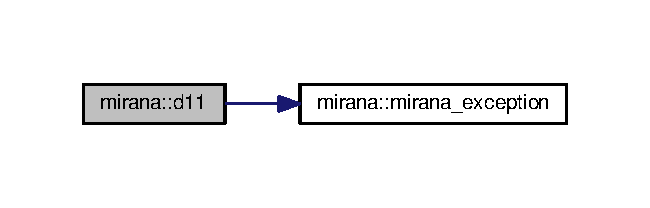
\includegraphics[width=312pt]{classmirana_ab9b1e7b5e38c6a020e05196b452e6d02_cgraph}
\end{center}
\end{figure}




Here is the caller graph for this function\-:
\nopagebreak
\begin{figure}[H]
\begin{center}
\leavevmode
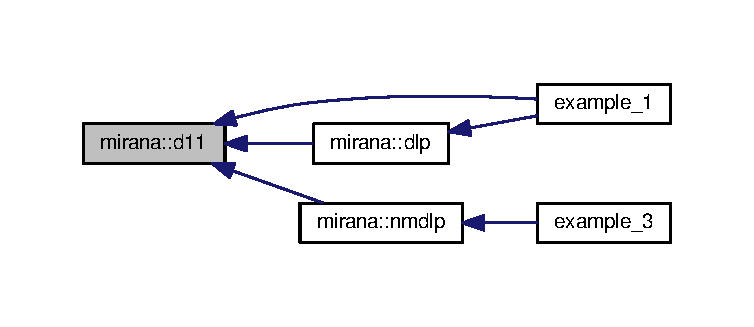
\includegraphics[width=350pt]{classmirana_ab9b1e7b5e38c6a020e05196b452e6d02_icgraph}
\end{center}
\end{figure}


\hypertarget{classmirana_ae9ee4058ea2b6238b6b745e4468f6a8e}{\index{mirana@{mirana}!d12@{d12}}
\index{d12@{d12}!mirana@{mirana}}
\subsubsection[{d12}]{\setlength{\rightskip}{0pt plus 5cm}subroutine mirana\-::d12 (
\begin{DoxyParamCaption}
\item[{double precision, dimension(\-:,\-:), intent(in), allocatable}]{phi, }
\item[{double precision, intent(in)}]{h1, }
\item[{double precision, intent(in)}]{h2, }
\item[{double precision, dimension(\-:,\-:), intent(inout), allocatable}]{phi\-\_\-xy}
\end{DoxyParamCaption}
)}}\label{classmirana_ae9ee4058ea2b6238b6b745e4468f6a8e}


Comopute the mixed second order derivative using central difference. 


\begin{DoxyParams}{Parameters}
{\em phi} & N1-\/by-\/\-N2 matrix. \\
\hline
{\em h1} & real number, step size 1. \\
\hline
{\em h2} & real number, step size 2. \\
\hline
{\em phi\-\_\-xy} & real N1-\/by-\/\-N2 matrix, only points ranged in \mbox{[}2\-:(N1-\/1)\mbox{]}X\mbox{[}2\-:(N2-\/1)\mbox{]} are updated. \\
\hline
\end{DoxyParams}


Here is the call graph for this function\-:\nopagebreak
\begin{figure}[H]
\begin{center}
\leavevmode
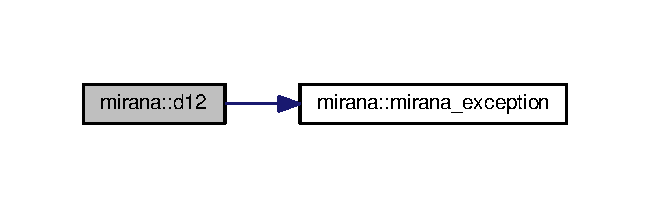
\includegraphics[width=312pt]{classmirana_ae9ee4058ea2b6238b6b745e4468f6a8e_cgraph}
\end{center}
\end{figure}




Here is the caller graph for this function\-:
\nopagebreak
\begin{figure}[H]
\begin{center}
\leavevmode
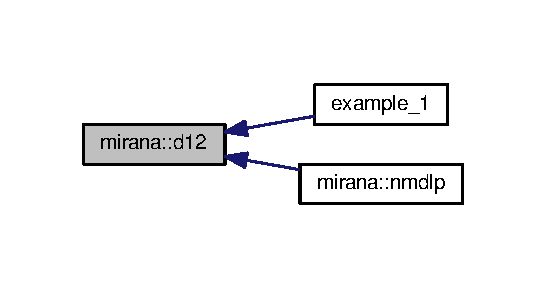
\includegraphics[width=350pt]{classmirana_ae9ee4058ea2b6238b6b745e4468f6a8e_icgraph}
\end{center}
\end{figure}


\hypertarget{classmirana_acc84c99770972f6328e89ac04ac67153}{\index{mirana@{mirana}!d1h1@{d1h1}}
\index{d1h1@{d1h1}!mirana@{mirana}}
\subsubsection[{d1h1}]{\setlength{\rightskip}{0pt plus 5cm}subroutine mirana\-::d1h1 (
\begin{DoxyParamCaption}
\item[{double precision, dimension(\-:,\-:), intent(in), allocatable}]{phi, }
\item[{double precision, intent(in)}]{h, }
\item[{double precision, dimension(\-:,\-:), intent(inout), allocatable}]{phi\-\_\-1h}
\end{DoxyParamCaption}
)}}\label{classmirana_acc84c99770972f6328e89ac04ac67153}


Compute the derivative along the 1st direction at the 1st kind of half points using central difference. 


\begin{DoxyParams}{Parameters}
{\em phi} & real N1-\/by-\/\-N2 matrix. \\
\hline
{\em h} & real number, step size. \\
\hline
\end{DoxyParams}
\begin{DoxyReturn}{Returns}
phi\-\_\-1h, real N1-\/by-\/\-N2 matrix, the (i,j) element stores the derivative at (i+1/2,j), only \mbox{[}1\-:N1-\/1\mbox{]}X\mbox{[}1\-:N2\mbox{]} part is used. 
\end{DoxyReturn}


Here is the call graph for this function\-:\nopagebreak
\begin{figure}[H]
\begin{center}
\leavevmode
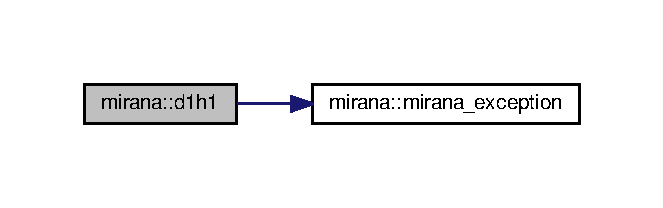
\includegraphics[width=318pt]{classmirana_acc84c99770972f6328e89ac04ac67153_cgraph}
\end{center}
\end{figure}




Here is the caller graph for this function\-:
\nopagebreak
\begin{figure}[H]
\begin{center}
\leavevmode
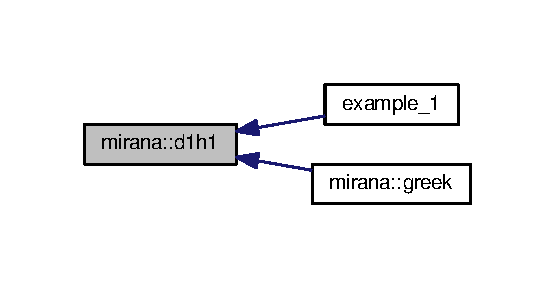
\includegraphics[width=350pt]{classmirana_acc84c99770972f6328e89ac04ac67153_icgraph}
\end{center}
\end{figure}


\hypertarget{classmirana_a9d6168761271912ebfea872e9f322cdc}{\index{mirana@{mirana}!d1h2@{d1h2}}
\index{d1h2@{d1h2}!mirana@{mirana}}
\subsubsection[{d1h2}]{\setlength{\rightskip}{0pt plus 5cm}subroutine mirana\-::d1h2 (
\begin{DoxyParamCaption}
\item[{double precision, dimension(\-:,\-:), intent(in), allocatable}]{phi, }
\item[{double precision, intent(in)}]{h, }
\item[{double precision, dimension(\-:,\-:), intent(inout), allocatable}]{phi\-\_\-1h}
\end{DoxyParamCaption}
)}}\label{classmirana_a9d6168761271912ebfea872e9f322cdc}


Compute the derivative along the 1st direction at the 2nd kind of half points using central difference. 


\begin{DoxyParams}{Parameters}
{\em phi} & real N1-\/by-\/\-N2 matrix. \\
\hline
{\em h} & real number, step size (h1). \\
\hline
\end{DoxyParams}
\begin{DoxyReturn}{Returns}
phi\-\_\-1h, real N1-\/by-\/\-N2 matrix, the (i,j) element stores the derivative at (i,j+1/2), only \mbox{[}2\-:N1-\/1\mbox{]}X\mbox{[}1\-:N2-\/1\mbox{]} part is used. 
\end{DoxyReturn}


Here is the call graph for this function\-:\nopagebreak
\begin{figure}[H]
\begin{center}
\leavevmode
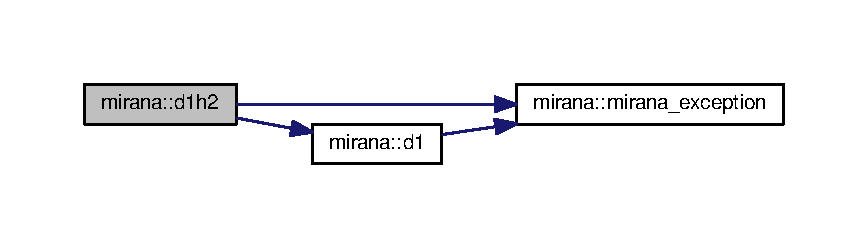
\includegraphics[width=350pt]{classmirana_a9d6168761271912ebfea872e9f322cdc_cgraph}
\end{center}
\end{figure}




Here is the caller graph for this function\-:
\nopagebreak
\begin{figure}[H]
\begin{center}
\leavevmode
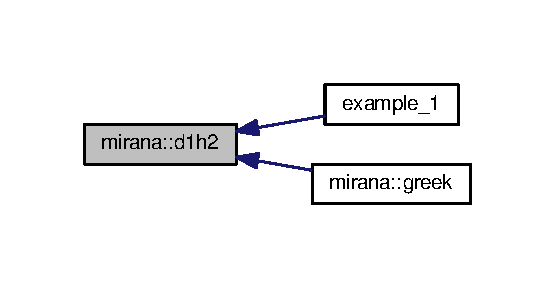
\includegraphics[width=350pt]{classmirana_a9d6168761271912ebfea872e9f322cdc_icgraph}
\end{center}
\end{figure}


\hypertarget{classmirana_a21348ffe170eafc6fc2a009256b1b6e3}{\index{mirana@{mirana}!d2@{d2}}
\index{d2@{d2}!mirana@{mirana}}
\subsubsection[{d2}]{\setlength{\rightskip}{0pt plus 5cm}subroutine mirana\-::d2 (
\begin{DoxyParamCaption}
\item[{double precision, dimension(\-:,\-:), intent(in), allocatable}]{phi, }
\item[{double precision, intent(in)}]{h, }
\item[{double precision, dimension(\-:,\-:), intent(inout), allocatable}]{phi\-\_\-y}
\end{DoxyParamCaption}
)}}\label{classmirana_a21348ffe170eafc6fc2a009256b1b6e3}


Differentiate with respect to the second dimension using central difference. 


\begin{DoxyParams}{Parameters}
{\em phi} & real N1-\/by-\/\-N2 matrix \\
\hline
{\em h} & real number, step size. \\
\hline
\end{DoxyParams}
\begin{DoxyReturn}{Returns}
phi\-\_\-y real N1-\/by-\/\-N2 matrix, only points ranged in \mbox{[}1\-:N1\mbox{]}X\mbox{[}2\-:(N2-\/1)\mbox{]} are updated. 
\end{DoxyReturn}


Here is the call graph for this function\-:\nopagebreak
\begin{figure}[H]
\begin{center}
\leavevmode
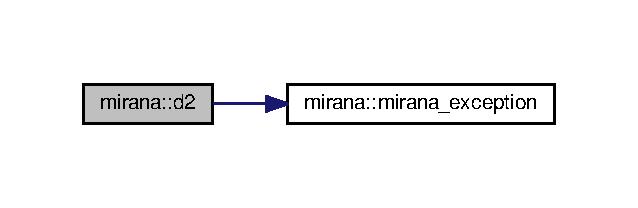
\includegraphics[width=306pt]{classmirana_a21348ffe170eafc6fc2a009256b1b6e3_cgraph}
\end{center}
\end{figure}




Here is the caller graph for this function\-:
\nopagebreak
\begin{figure}[H]
\begin{center}
\leavevmode
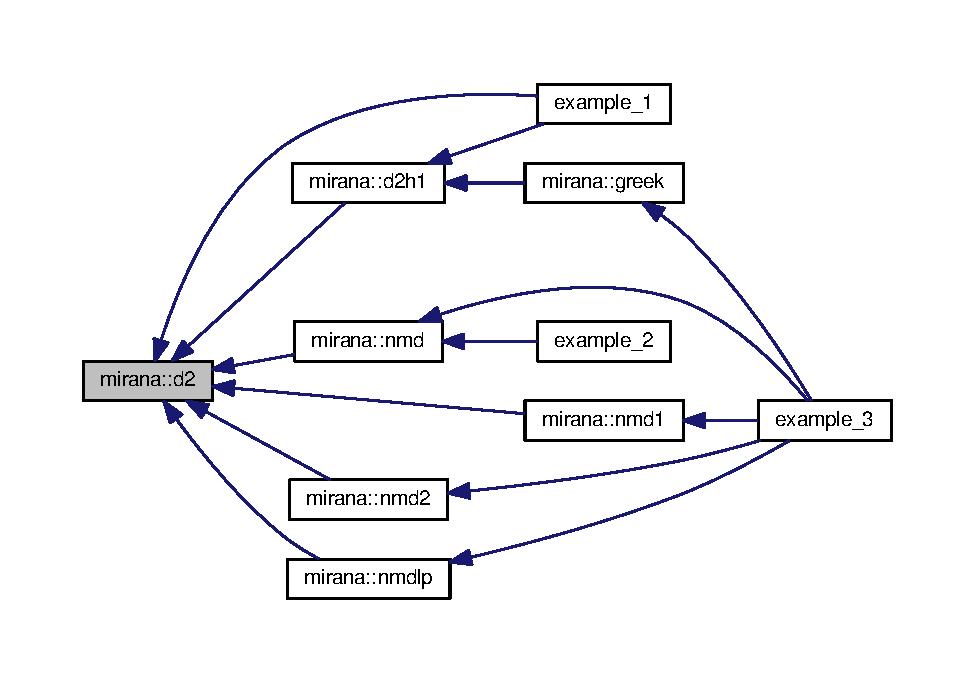
\includegraphics[width=350pt]{classmirana_a21348ffe170eafc6fc2a009256b1b6e3_icgraph}
\end{center}
\end{figure}


\hypertarget{classmirana_a9161b0947ddd188ac99d9246a1d81aed}{\index{mirana@{mirana}!d22@{d22}}
\index{d22@{d22}!mirana@{mirana}}
\subsubsection[{d22}]{\setlength{\rightskip}{0pt plus 5cm}subroutine mirana\-::d22 (
\begin{DoxyParamCaption}
\item[{double precision, dimension(\-:,\-:), intent(in), allocatable}]{phi, }
\item[{double precision, intent(in)}]{h, }
\item[{double precision, dimension(\-:,\-:), intent(inout), allocatable}]{phi\-\_\-yy}
\end{DoxyParamCaption}
)}}\label{classmirana_a9161b0947ddd188ac99d9246a1d81aed}


Compute the second order derivative along the second dimension using central difference. 


\begin{DoxyParams}{Parameters}
{\em phi} & N1-\/by-\/\-N2 real matrix. \\
\hline
{\em h} & real number, step size. \\
\hline
{\em phi\-\_\-yy} & real N1-\/by-\/\-N2 matrix, only points ranged in \mbox{[}1\-:N1\mbox{]}X\mbox{[}2\-:(N2-\/1)\mbox{]} are updated. \\
\hline
\end{DoxyParams}


Here is the call graph for this function\-:\nopagebreak
\begin{figure}[H]
\begin{center}
\leavevmode
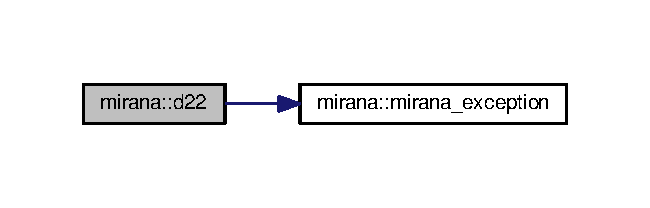
\includegraphics[width=312pt]{classmirana_a9161b0947ddd188ac99d9246a1d81aed_cgraph}
\end{center}
\end{figure}




Here is the caller graph for this function\-:
\nopagebreak
\begin{figure}[H]
\begin{center}
\leavevmode
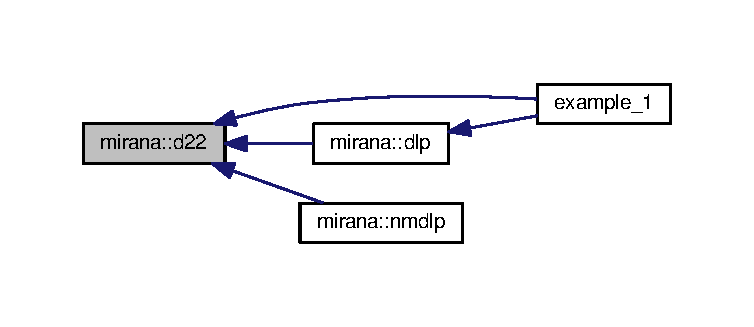
\includegraphics[width=350pt]{classmirana_a9161b0947ddd188ac99d9246a1d81aed_icgraph}
\end{center}
\end{figure}


\hypertarget{classmirana_a9341f957abd27c5132c557ae873055bd}{\index{mirana@{mirana}!d2h1@{d2h1}}
\index{d2h1@{d2h1}!mirana@{mirana}}
\subsubsection[{d2h1}]{\setlength{\rightskip}{0pt plus 5cm}subroutine mirana\-::d2h1 (
\begin{DoxyParamCaption}
\item[{double precision, dimension(\-:,\-:), intent(in), allocatable}]{phi, }
\item[{double precision, intent(in)}]{h, }
\item[{double precision, dimension(\-:,\-:), intent(inout), allocatable}]{phi\-\_\-2h}
\end{DoxyParamCaption}
)}}\label{classmirana_a9341f957abd27c5132c557ae873055bd}


Compute the derivative along the 2nd direction at the 1st kind of half points using central difference. 


\begin{DoxyParams}{Parameters}
{\em phi} & real N1-\/by-\/\-N2 matrix. \\
\hline
{\em h} & real number, step size (h2). \\
\hline
\end{DoxyParams}
\begin{DoxyReturn}{Returns}
phi\-\_\-2h, real N1-\/by-\/\-N2 matrix, the (i,j) element stores the derivative at (i+1/2,j), only \mbox{[}1\-:N1-\/1\mbox{]}X\mbox{[}2\-:N2-\/1\mbox{]} part is used. 
\end{DoxyReturn}


Here is the call graph for this function\-:\nopagebreak
\begin{figure}[H]
\begin{center}
\leavevmode
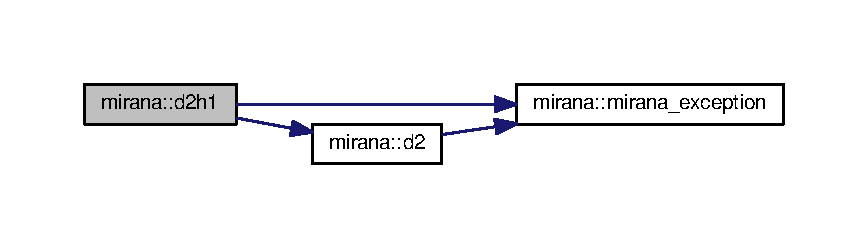
\includegraphics[width=350pt]{classmirana_a9341f957abd27c5132c557ae873055bd_cgraph}
\end{center}
\end{figure}




Here is the caller graph for this function\-:
\nopagebreak
\begin{figure}[H]
\begin{center}
\leavevmode
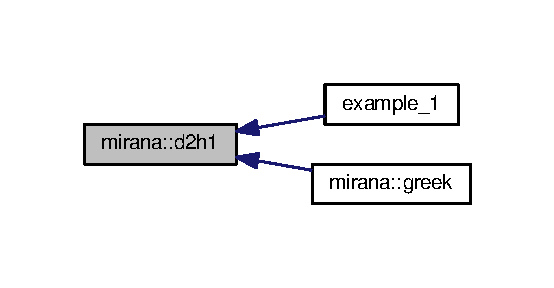
\includegraphics[width=350pt]{classmirana_a9341f957abd27c5132c557ae873055bd_icgraph}
\end{center}
\end{figure}


\hypertarget{classmirana_a4f47c93df57dd51d1414b2514fd1b339}{\index{mirana@{mirana}!d2h2@{d2h2}}
\index{d2h2@{d2h2}!mirana@{mirana}}
\subsubsection[{d2h2}]{\setlength{\rightskip}{0pt plus 5cm}subroutine mirana\-::d2h2 (
\begin{DoxyParamCaption}
\item[{double precision, dimension(\-:,\-:), intent(in), allocatable}]{phi, }
\item[{double precision, intent(in)}]{h, }
\item[{double precision, dimension(\-:,\-:), intent(inout), allocatable}]{phi\-\_\-2h}
\end{DoxyParamCaption}
)}}\label{classmirana_a4f47c93df57dd51d1414b2514fd1b339}


Compute the derivative along the 2nd direction at the 2nd kind of half points using central difference. 


\begin{DoxyParams}{Parameters}
{\em phi} & real N1-\/by-\/\-N2 matrix. \\
\hline
{\em h} & real number, step size. \\
\hline
\end{DoxyParams}
\begin{DoxyReturn}{Returns}
phi\-\_\-2h, real N1-\/by-\/\-N2 matrix, the (i,j) element stores the derivative at (i,j+1/2), only \mbox{[}1\-:N1\mbox{]}X\mbox{[}1\-:N2-\/1\mbox{]} part is used. 
\end{DoxyReturn}


Here is the call graph for this function\-:\nopagebreak
\begin{figure}[H]
\begin{center}
\leavevmode
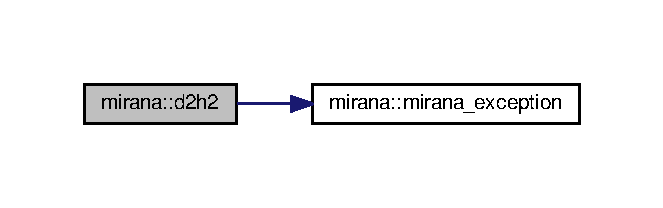
\includegraphics[width=318pt]{classmirana_a4f47c93df57dd51d1414b2514fd1b339_cgraph}
\end{center}
\end{figure}




Here is the caller graph for this function\-:
\nopagebreak
\begin{figure}[H]
\begin{center}
\leavevmode
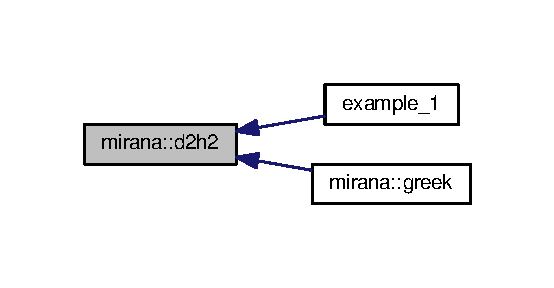
\includegraphics[width=350pt]{classmirana_a4f47c93df57dd51d1414b2514fd1b339_icgraph}
\end{center}
\end{figure}


\hypertarget{classmirana_a353bce8a93046cd8fd25021634d6503e}{\index{mirana@{mirana}!dlp@{dlp}}
\index{dlp@{dlp}!mirana@{mirana}}
\subsubsection[{dlp}]{\setlength{\rightskip}{0pt plus 5cm}subroutine mirana\-::dlp (
\begin{DoxyParamCaption}
\item[{double precision, dimension(\-:,\-:), intent(in), allocatable}]{phi, }
\item[{double precision, intent(in)}]{h1, }
\item[{double precision, intent(in)}]{h2, }
\item[{double precision, dimension(\-:,\-:), intent(inout), allocatable}]{phi\-\_\-lp}
\end{DoxyParamCaption}
)}}\label{classmirana_a353bce8a93046cd8fd25021634d6503e}


Compute Laplacian using central difference. 


\begin{DoxyParams}{Parameters}
{\em phi} & N1-\/by-\/\-N2 matrix. \\
\hline
{\em h1} & real number, step size 1. \\
\hline
{\em h2} & real number, step size 2. \\
\hline
{\em phi\-\_\-lp} & real N1-\/by-\/\-N2 matrix, only points ranged in \mbox{[}2\-:(N1-\/1)\mbox{]}X\mbox{[}2\-:(N2-\/1)\mbox{]} are updated. \\
\hline
\end{DoxyParams}


Here is the call graph for this function\-:\nopagebreak
\begin{figure}[H]
\begin{center}
\leavevmode
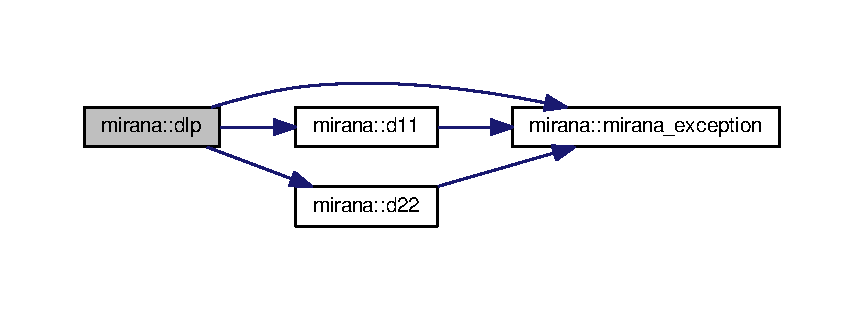
\includegraphics[width=350pt]{classmirana_a353bce8a93046cd8fd25021634d6503e_cgraph}
\end{center}
\end{figure}




Here is the caller graph for this function\-:\nopagebreak
\begin{figure}[H]
\begin{center}
\leavevmode
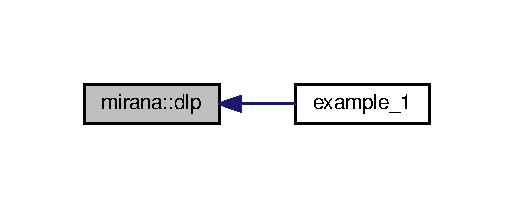
\includegraphics[width=246pt]{classmirana_a353bce8a93046cd8fd25021634d6503e_icgraph}
\end{center}
\end{figure}


\hypertarget{classmirana_a7530ea2e7b2dfe85f3a088d24de59f1d}{\index{mirana@{mirana}!greek@{greek}}
\index{greek@{greek}!mirana@{mirana}}
\subsubsection[{greek}]{\setlength{\rightskip}{0pt plus 5cm}subroutine mirana\-::greek (
\begin{DoxyParamCaption}
\item[{double precision, dimension(\-:,\-:), intent(in), allocatable}]{mx, }
\item[{double precision, dimension(\-:,\-:), intent(in), allocatable}]{my, }
\item[{double precision, dimension(\-:,\-:), intent(in), allocatable}]{xix, }
\item[{double precision, dimension(\-:,\-:), intent(in), allocatable}]{xiy, }
\item[{double precision, dimension(\-:,\-:), intent(in), allocatable}]{etx, }
\item[{double precision, dimension(\-:,\-:), intent(in), allocatable}]{ety, }
\item[{double precision, intent(in)}]{h1, }
\item[{double precision, intent(in)}]{h2, }
\item[{double precision, dimension(\-:,\-:), intent(inout), allocatable}]{alp, }
\item[{double precision, dimension(\-:,\-:), intent(inout), allocatable}]{bet}
\end{DoxyParamCaption}
)}}\label{classmirana_a7530ea2e7b2dfe85f3a088d24de59f1d}


Compute the two coefficients for transformed laplacian $\alpha,\beta$. 


\begin{DoxyParams}{Parameters}
{\em mx} & real N1-\/by-\/\-N2 matrix, mesh coordinates -\/ x. \\
\hline
{\em my} & real N1-\/by-\/\-N2 matrix, mesh coordinates -\/ y. \\
\hline
{\em xix} & real N1-\/by-\/\-N2 matrix, $\partial\xi/\partial x$. \\
\hline
{\em xiy} & real N1-\/by-\/\-N2 matrix, $\partial\xi/\partial y$. \\
\hline
{\em etx} & real N1-\/by-\/\-N2 matrix, $\partial\eta/\partial x$. \\
\hline
{\em ety} & real N1-\/by-\/\-N2 matrix, $\partial\eta/\partial y$. \\
\hline
{\em h1} & real number, step size in the first direction. \\
\hline
{\em h2} & real number, step size in the second direction. \\
\hline
\end{DoxyParams}
\begin{DoxyReturn}{Returns}
alp real N1-\/by-\/\-N2 matrix, the $\alpha$, only \mbox{[}2\-:N1-\/1\mbox{]}X\mbox{[}2\-:N2-\/1\mbox{]} is used. 

bet real N1-\/by-\/\-N2 matrix, the $\beta$, only \mbox{[}2\-:N1-\/1\mbox{]}X\mbox{[}2\-:N2-\/1\mbox{]} is used. 
\end{DoxyReturn}


Here is the call graph for this function\-:\nopagebreak
\begin{figure}[H]
\begin{center}
\leavevmode
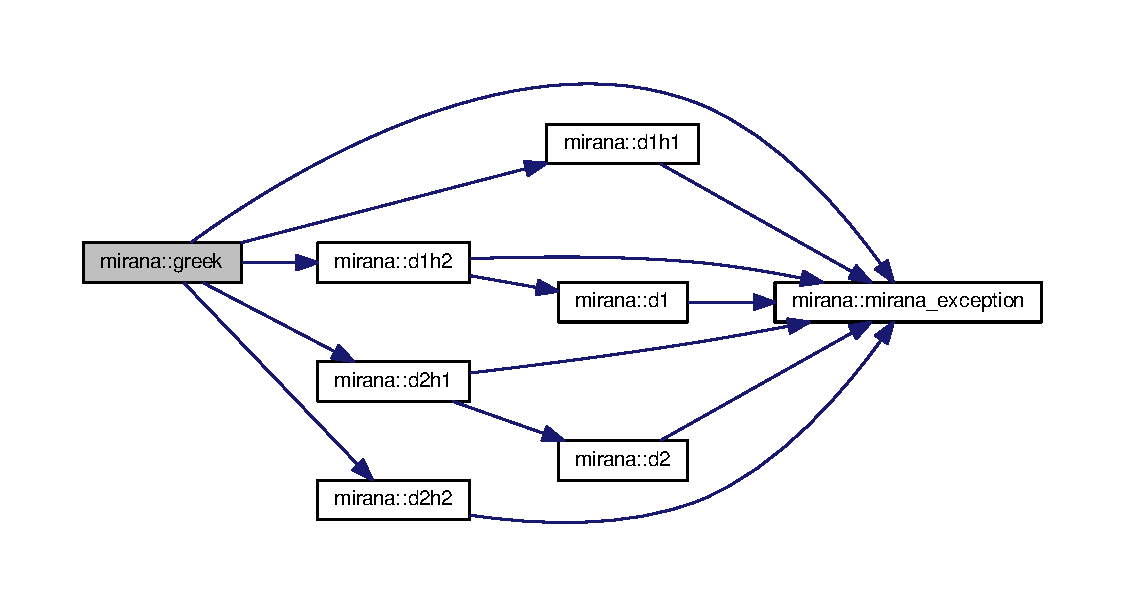
\includegraphics[width=350pt]{classmirana_a7530ea2e7b2dfe85f3a088d24de59f1d_cgraph}
\end{center}
\end{figure}




Here is the caller graph for this function\-:
\nopagebreak
\begin{figure}[H]
\begin{center}
\leavevmode
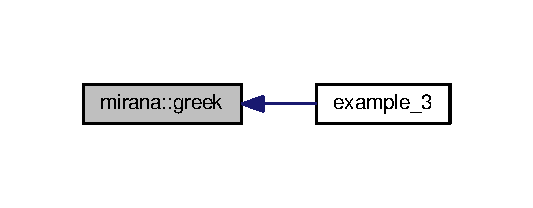
\includegraphics[width=256pt]{classmirana_a7530ea2e7b2dfe85f3a088d24de59f1d_icgraph}
\end{center}
\end{figure}


\hypertarget{classmirana_a65a514d206d0e8ae53253938d2aff553}{\index{mirana@{mirana}!mbc\-\_\-d@{mbc\-\_\-d}}
\index{mbc\-\_\-d@{mbc\-\_\-d}!mirana@{mirana}}
\subsubsection[{mbc\-\_\-d}]{\setlength{\rightskip}{0pt plus 5cm}subroutine mirana\-::mbc\-\_\-d (
\begin{DoxyParamCaption}
\item[{double precision, dimension(\-:,\-:), intent(inout), allocatable}]{x1, }
\item[{double precision, dimension(\-:,\-:), intent(inout), allocatable}]{x2, }
\item[{double precision, dimension(\-:,\-:), intent(inout), allocatable}]{y1, }
\item[{double precision, dimension(\-:,\-:), intent(inout), allocatable}]{y2}
\end{DoxyParamCaption}
)}}\label{classmirana_a65a514d206d0e8ae53253938d2aff553}


(Mesh Boundary Condition for Derivatives) Set the boundary condition of the moving mesh. 

\begin{DoxyNote}{Note}
Be sure to call Mirana\-::d1 and Mirana\-::d2 on the mesh before calling this subroutine! 
\end{DoxyNote}

\begin{DoxyParams}{Parameters}
{\em x1,N1-\/by-\/\-N2} & real array, resulted from call d1(mx,hxi,x1). \\
\hline
{\em x2,N1-\/by-\/\-N2} & real array, resulted from call d2(mx,het,x2). \\
\hline
{\em y1,N1-\/by-\/\-N2} & real array, resulted from call d1(my,hxi,y1). \\
\hline
{\em y2,N1-\/by-\/\-N2} & real array, resulted from call d2(my,het,y2). \\
\hline
\end{DoxyParams}

\begin{DoxyItemize}
\item Use uniform mesh at left/right boundary.
\item $\xi$-\/mesh is parallel to the wall at floor/ceiling. 
\end{DoxyItemize}

Here is the call graph for this function\-:\nopagebreak
\begin{figure}[H]
\begin{center}
\leavevmode
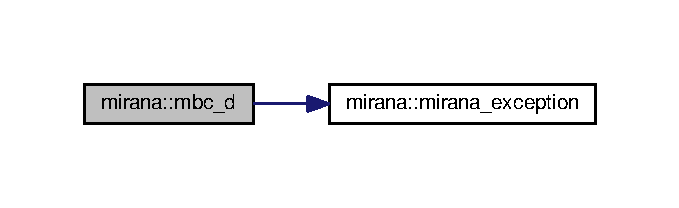
\includegraphics[width=326pt]{classmirana_a65a514d206d0e8ae53253938d2aff553_cgraph}
\end{center}
\end{figure}




Here is the caller graph for this function\-:
\nopagebreak
\begin{figure}[H]
\begin{center}
\leavevmode
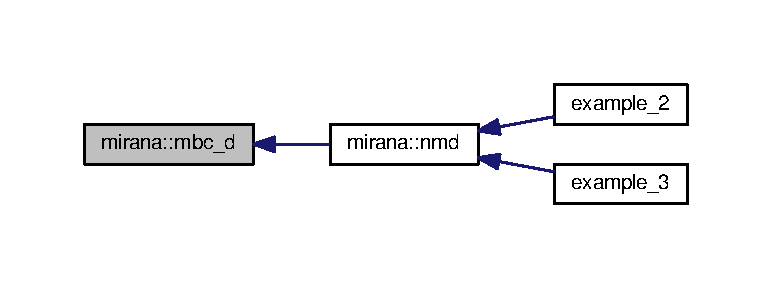
\includegraphics[width=350pt]{classmirana_a65a514d206d0e8ae53253938d2aff553_icgraph}
\end{center}
\end{figure}


\hypertarget{classmirana_ab002a22665f70b4c65bdcf70ac96d768}{\index{mirana@{mirana}!mirana\-\_\-exception@{mirana\-\_\-exception}}
\index{mirana\-\_\-exception@{mirana\-\_\-exception}!mirana@{mirana}}
\subsubsection[{mirana\-\_\-exception}]{\setlength{\rightskip}{0pt plus 5cm}subroutine mirana\-::mirana\-\_\-exception (
\begin{DoxyParamCaption}
\item[{character, dimension(128), intent(in)}]{message}
\end{DoxyParamCaption}
)}}\label{classmirana_ab002a22665f70b4c65bdcf70ac96d768}


Handling exceptions. 


\begin{DoxyParams}{Parameters}
{\em n} & integer, exit code. \\
\hline
{\em message} & string with length 128, error message. \\
\hline
\end{DoxyParams}


Here is the caller graph for this function\-:
\nopagebreak
\begin{figure}[H]
\begin{center}
\leavevmode
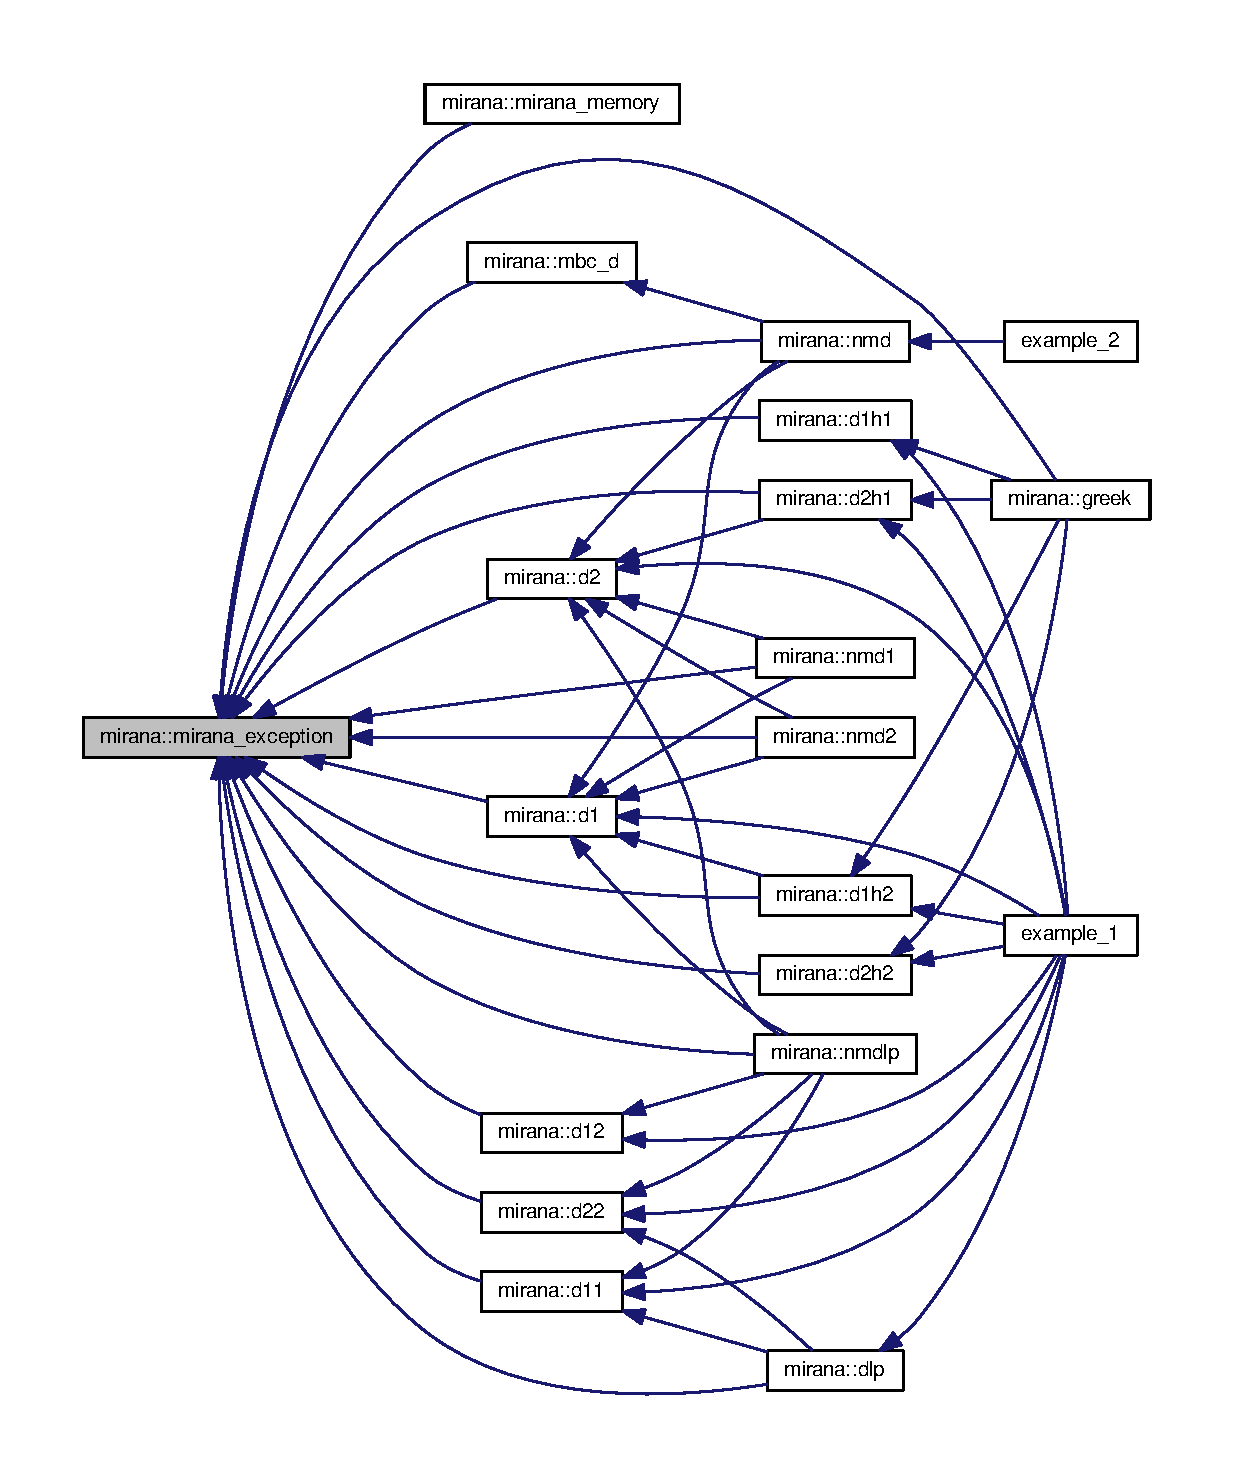
\includegraphics[width=350pt]{classmirana_ab002a22665f70b4c65bdcf70ac96d768_icgraph}
\end{center}
\end{figure}


\hypertarget{classmirana_acccf612b21e3e65bd3a78131c48afe2b}{\index{mirana@{mirana}!mirana\-\_\-memory@{mirana\-\_\-memory}}
\index{mirana\-\_\-memory@{mirana\-\_\-memory}!mirana@{mirana}}
\subsubsection[{mirana\-\_\-memory}]{\setlength{\rightskip}{0pt plus 5cm}subroutine mirana\-::mirana\-\_\-memory (
\begin{DoxyParamCaption}
\item[{double precision, dimension(\-:,\-:), intent(inout), allocatable}]{name, }
\item[{integer, intent(in)}]{dim1, }
\item[{integer, intent(in)}]{dim2}
\end{DoxyParamCaption}
)}}\label{classmirana_acccf612b21e3e65bd3a78131c48afe2b}


Allocate memory for new arrays. 


\begin{DoxyParams}{Parameters}
{\em name} & real allocatable 2-\/dim array (not allocated). \\
\hline
{\em dim} & integer, dimension. \\
\hline
\end{DoxyParams}
\begin{DoxyReturn}{Returns}
name dim1-\/by-\/dim2 real array with memory allocated. 
\end{DoxyReturn}


Here is the call graph for this function\-:\nopagebreak
\begin{figure}[H]
\begin{center}
\leavevmode
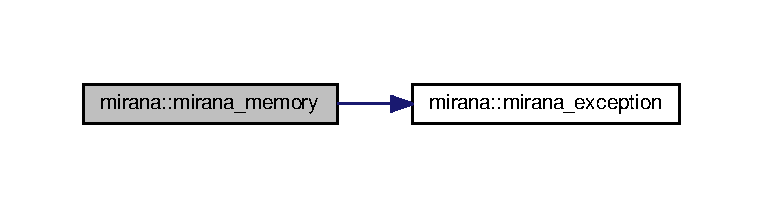
\includegraphics[width=350pt]{classmirana_acccf612b21e3e65bd3a78131c48afe2b_cgraph}
\end{center}
\end{figure}


\hypertarget{classmirana_a53c223d4530275ef3fc6a5820f5b0990}{\index{mirana@{mirana}!nmd@{nmd}}
\index{nmd@{nmd}!mirana@{mirana}}
\subsubsection[{nmd}]{\setlength{\rightskip}{0pt plus 5cm}subroutine mirana\-::nmd (
\begin{DoxyParamCaption}
\item[{double precision, dimension(\-:,\-:), intent(in), allocatable}]{mx, }
\item[{double precision, dimension(\-:,\-:), intent(in), allocatable}]{my, }
\item[{double precision, intent(in)}]{hxi, }
\item[{double precision, intent(in)}]{het, }
\item[{double precision, dimension(\-:,\-:), intent(inout), allocatable}]{jcb, }
\item[{double precision, dimension(\-:,\-:), intent(inout), allocatable}]{xi\-\_\-x, }
\item[{double precision, dimension(\-:,\-:), intent(inout), allocatable}]{xi\-\_\-y, }
\item[{double precision, dimension(\-:,\-:), intent(inout), allocatable}]{et\-\_\-x, }
\item[{double precision, dimension(\-:,\-:), intent(inout), allocatable}]{et\-\_\-y}
\end{DoxyParamCaption}
)}}\label{classmirana_a53c223d4530275ef3fc6a5820f5b0990}


(Non-\/conservative Mesh Differentiation) Compute derivatives of mesh grid with respect to computational space and inverse using non-\/conservative form central difference. 

\begin{DoxyNote}{Note}
\hyperlink{classmirana_a53c223d4530275ef3fc6a5820f5b0990}{nmd()} and \hyperlink{classmirana_a7530ea2e7b2dfe85f3a088d24de59f1d}{greek()} computes all fundamental coefficients in non-\/conservative form. 
\end{DoxyNote}

\begin{DoxyParams}{Parameters}
{\em mx} & N1-\/by-\/\-N2 real matrix, x-\/coordinate of mesh grid (fully determined). \\
\hline
{\em my} & N1-\/by-\/\-N2 real matrix, y-\/coordinate of mesh grid (fully determined). \\
\hline
{\em hxi} & real number, step size in computational domain along $\xi$ direction. \\
\hline
{\em het} & real number, step size in computational domain along $\eta$ direction. \\
\hline
\end{DoxyParams}
\begin{DoxyReturn}{Returns}
jcb real N1-\/by-\/\-N2 matrix, the Jacobian $J$. 

xi\-\_\-x real N1-\/by-\/\-N2 matrix, $\partial\xi/\partial x$. 

xi\-\_\-y real N1-\/by-\/\-N2 matrix, $\partial\xi/\partial y$. 

et\-\_\-x real N1-\/by-\/\-N2 matrix, $\partial\eta/\partial x$. 

et\-\_\-y real N1-\/by-\/\-N2 matrix, $\partial\eta/\partial y$. 
\end{DoxyReturn}


Here is the call graph for this function\-:\nopagebreak
\begin{figure}[H]
\begin{center}
\leavevmode
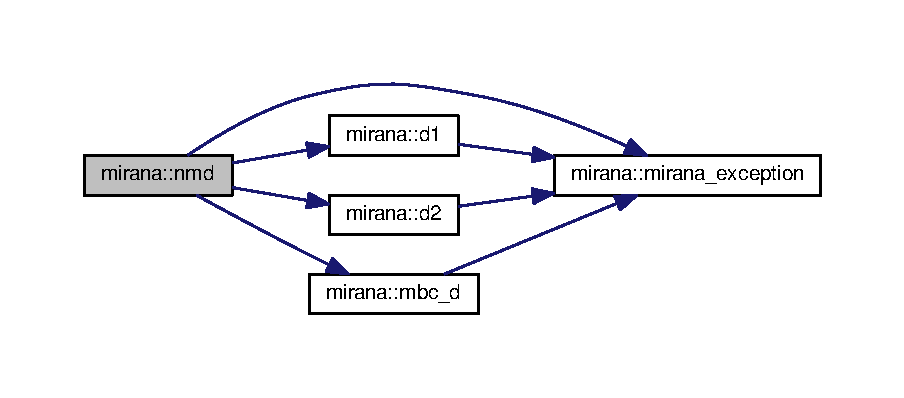
\includegraphics[width=350pt]{classmirana_a53c223d4530275ef3fc6a5820f5b0990_cgraph}
\end{center}
\end{figure}




Here is the caller graph for this function\-:
\nopagebreak
\begin{figure}[H]
\begin{center}
\leavevmode
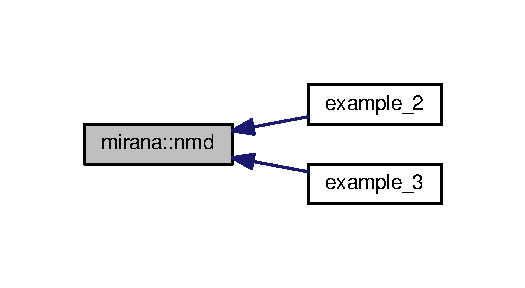
\includegraphics[width=252pt]{classmirana_a53c223d4530275ef3fc6a5820f5b0990_icgraph}
\end{center}
\end{figure}


\hypertarget{classmirana_a6b48fffbaaa6f2256928cd73d8891261}{\index{mirana@{mirana}!nmd1@{nmd1}}
\index{nmd1@{nmd1}!mirana@{mirana}}
\subsubsection[{nmd1}]{\setlength{\rightskip}{0pt plus 5cm}subroutine mirana\-::nmd1 (
\begin{DoxyParamCaption}
\item[{double precision, dimension(\-:,\-:), intent(in), allocatable}]{phi, }
\item[{double precision, dimension(\-:,\-:), intent(in), allocatable}]{xix, }
\item[{double precision, dimension(\-:,\-:), intent(in), allocatable}]{etx, }
\item[{double precision, intent(in)}]{h1, }
\item[{double precision, intent(in)}]{h2, }
\item[{double precision, dimension(\-:,\-:), intent(inout), allocatable}]{phi\-\_\-x}
\end{DoxyParamCaption}
)}}\label{classmirana_a6b48fffbaaa6f2256928cd73d8891261}


(Non-\/conservative Mesh D1) Compute $\partial\phi/\partial x$ using mesh variables 


\begin{DoxyParams}{Parameters}
{\em phi} & N1-\/by-\/\-N2 real matrix. \\
\hline
{\em xix} & N1-\/by-\/\-N2 real matrix, $\partial\xi\partial x$. \\
\hline
{\em etx} & N1-\/by-\/\-N2 real matrix, $\partial\eta\partial x$. \\
\hline
{\em h1} & real number, step size in $\xi$ axis. \\
\hline
{\em h2} & real number, step size in $\eta$ axis. \\
\hline
\end{DoxyParams}
\begin{DoxyReturn}{Returns}
phi\-\_\-x N1-\/by-\/\-N2 real matrix, only \mbox{[}2\-:N1-\/1\mbox{]}X\mbox{[}2\-:N2-\/1\mbox{]} are used. 
\end{DoxyReturn}


Here is the call graph for this function\-:\nopagebreak
\begin{figure}[H]
\begin{center}
\leavevmode
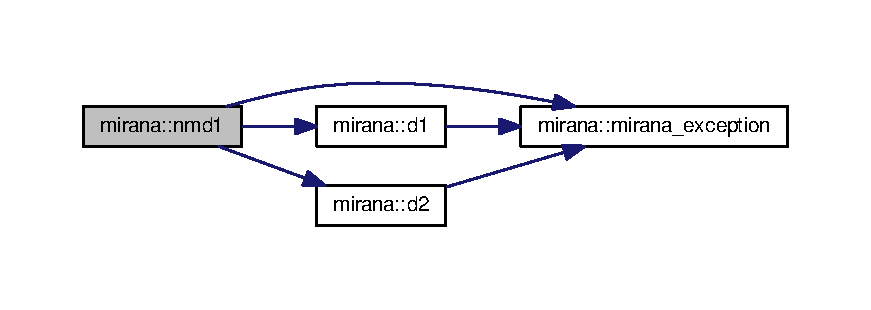
\includegraphics[width=350pt]{classmirana_a6b48fffbaaa6f2256928cd73d8891261_cgraph}
\end{center}
\end{figure}




Here is the caller graph for this function\-:
\nopagebreak
\begin{figure}[H]
\begin{center}
\leavevmode
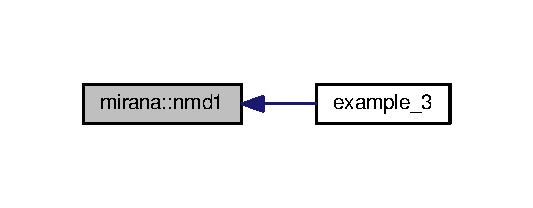
\includegraphics[width=256pt]{classmirana_a6b48fffbaaa6f2256928cd73d8891261_icgraph}
\end{center}
\end{figure}


\hypertarget{classmirana_a04bd9101c8bdc2f8b69892bd773f3055}{\index{mirana@{mirana}!nmd2@{nmd2}}
\index{nmd2@{nmd2}!mirana@{mirana}}
\subsubsection[{nmd2}]{\setlength{\rightskip}{0pt plus 5cm}subroutine mirana\-::nmd2 (
\begin{DoxyParamCaption}
\item[{double precision, dimension(\-:,\-:), intent(in), allocatable}]{phi, }
\item[{double precision, dimension(\-:,\-:), intent(in), allocatable}]{xiy, }
\item[{double precision, dimension(\-:,\-:), intent(in), allocatable}]{ety, }
\item[{double precision, intent(in)}]{h1, }
\item[{double precision, intent(in)}]{h2, }
\item[{double precision, dimension(\-:,\-:), intent(inout), allocatable}]{phi\-\_\-y}
\end{DoxyParamCaption}
)}}\label{classmirana_a04bd9101c8bdc2f8b69892bd773f3055}


(Non-\/conservative Mesh D2) Compute $\partial\phi/\partial y$ using mesh variables 


\begin{DoxyParams}{Parameters}
{\em phi} & N1-\/by-\/\-N2 real matrix. \\
\hline
{\em xiy} & N1-\/by-\/\-N2 real matrix, $\partial\xi\partial y$. \\
\hline
{\em ety} & N1-\/by-\/\-N2 real matrix, $\partial\eta\partial y$. \\
\hline
{\em h1} & real number, step size in $\xi$ axis. \\
\hline
{\em h2} & real number, step size in $\eta$ axis. \\
\hline
\end{DoxyParams}
\begin{DoxyReturn}{Returns}
phi\-\_\-y N1-\/by-\/\-N2 real matrix, only \mbox{[}2\-:N1-\/1\mbox{]}X\mbox{[}2\-:N2-\/1\mbox{]} are used. 
\end{DoxyReturn}


Here is the call graph for this function\-:\nopagebreak
\begin{figure}[H]
\begin{center}
\leavevmode
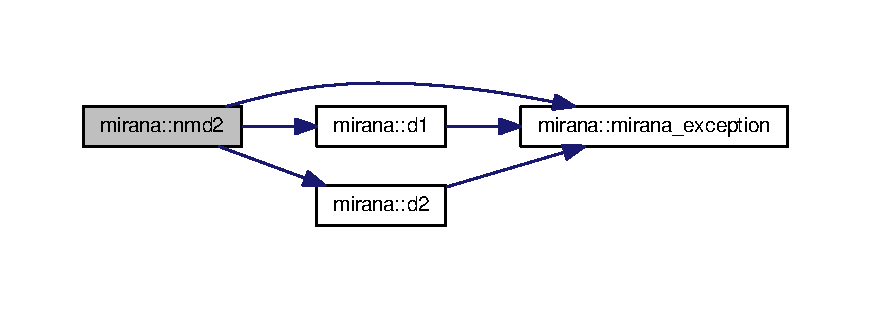
\includegraphics[width=350pt]{classmirana_a04bd9101c8bdc2f8b69892bd773f3055_cgraph}
\end{center}
\end{figure}




Here is the caller graph for this function\-:
\nopagebreak
\begin{figure}[H]
\begin{center}
\leavevmode
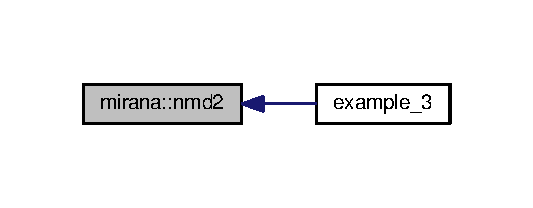
\includegraphics[width=256pt]{classmirana_a04bd9101c8bdc2f8b69892bd773f3055_icgraph}
\end{center}
\end{figure}


\hypertarget{classmirana_a503a76ad6fbdf28508f8d71786bed518}{\index{mirana@{mirana}!nmdlp@{nmdlp}}
\index{nmdlp@{nmdlp}!mirana@{mirana}}
\subsubsection[{nmdlp}]{\setlength{\rightskip}{0pt plus 5cm}subroutine mirana\-::nmdlp (
\begin{DoxyParamCaption}
\item[{double precision, dimension(\-:,\-:), intent(in), allocatable}]{phi, }
\item[{double precision, dimension(\-:,\-:), intent(in), allocatable}]{xix, }
\item[{double precision, dimension(\-:,\-:), intent(in), allocatable}]{xiy, }
\item[{double precision, dimension(\-:,\-:), intent(in), allocatable}]{etx, }
\item[{double precision, dimension(\-:,\-:), intent(in), allocatable}]{ety, }
\item[{double precision, dimension(\-:,\-:), intent(in), allocatable}]{alp, }
\item[{double precision, dimension(\-:,\-:), intent(in), allocatable}]{bet, }
\item[{double precision, intent(in)}]{h1, }
\item[{double precision, intent(in)}]{h2, }
\item[{double precision, dimension(\-:,\-:), intent(inout), allocatable}]{phi\-\_\-lp}
\end{DoxyParamCaption}
)}}\label{classmirana_a503a76ad6fbdf28508f8d71786bed518}


(Non-\/conservative Mesh D\-L\-P) Compute $\Delta\phi$ using mesh variables 


\begin{DoxyParams}{Parameters}
{\em phi} & N1-\/by-\/\-N2 real matrix. \\
\hline
{\em xix} & N1-\/by-\/\-N2 real matrix, $\partial\xi\partial x$. \\
\hline
{\em xiy} & N1-\/by-\/\-N2 real matrix, $\partial\xi\partial y$. \\
\hline
{\em etx} & N1-\/by-\/\-N2 real matrix, $\partial\eta\partial x$. \\
\hline
{\em ety} & N1-\/by-\/\-N2 real matrix, $\partial\eta\partial y$. \\
\hline
{\em alp} & N1-\/by-\/\-N2 real matrix, obtained from \hyperlink{classmirana_a7530ea2e7b2dfe85f3a088d24de59f1d}{greek()}. \\
\hline
{\em bet} & N1-\/by-\/\-N2 real matrix, obtained from \hyperlink{classmirana_a7530ea2e7b2dfe85f3a088d24de59f1d}{greek()}. \\
\hline
{\em h1} & real number, step size in $\xi$ axis. \\
\hline
{\em h2} & real number, step size in $\eta$ axis. \\
\hline
\end{DoxyParams}
\begin{DoxyReturn}{Returns}
phi\-\_\-lp N1-\/by-\/\-N2 real matrix, only \mbox{[}2\-:N1-\/1\mbox{]}X\mbox{[}2\-:N2-\/1\mbox{]} are used. 
\end{DoxyReturn}


Here is the call graph for this function\-:\nopagebreak
\begin{figure}[H]
\begin{center}
\leavevmode
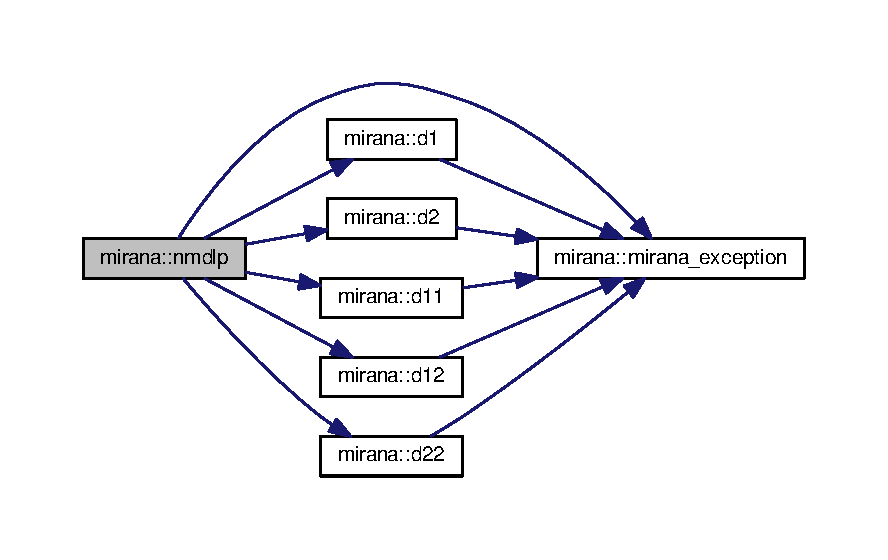
\includegraphics[width=350pt]{classmirana_a503a76ad6fbdf28508f8d71786bed518_cgraph}
\end{center}
\end{figure}




Here is the caller graph for this function\-:
\nopagebreak
\begin{figure}[H]
\begin{center}
\leavevmode
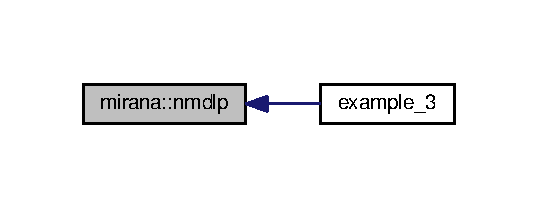
\includegraphics[width=258pt]{classmirana_a503a76ad6fbdf28508f8d71786bed518_icgraph}
\end{center}
\end{figure}


\hypertarget{classmirana_a9cbee1a318e5e828590c9ccaa51c8472}{\index{mirana@{mirana}!save\-\_\-mesh@{save\-\_\-mesh}}
\index{save\-\_\-mesh@{save\-\_\-mesh}!mirana@{mirana}}
\subsubsection[{save\-\_\-mesh}]{\setlength{\rightskip}{0pt plus 5cm}subroutine mirana\-::save\-\_\-mesh (
\begin{DoxyParamCaption}
\item[{double precision, dimension(\-:,\-:), intent(in), allocatable}]{mx, }
\item[{double precision, dimension(\-:,\-:), intent(in), allocatable}]{my}
\end{DoxyParamCaption}
)}}\label{classmirana_a9cbee1a318e5e828590c9ccaa51c8472}


Write mesh data into .dat file for plot. 


\begin{DoxyParams}{Parameters}
{\em mx} & real N1-\/by-\/\-N2 matrix, x-\/coodinates. \\
\hline
{\em my} & real N1-\/by-\/\-N2 matrix, x-\/coodinates. \\
\hline
\end{DoxyParams}
\begin{DoxyNote}{Note}
After generating mesh.\-dat, call the following command in Gnuplot\-:
\begin{DoxyItemize}
\item set view 0,0
\item splot \char`\"{}mesh.\-dat\char`\"{} using 1\-:2\-:3 with lines 
\end{DoxyItemize}
\end{DoxyNote}


Here is the caller graph for this function\-:\nopagebreak
\begin{figure}[H]
\begin{center}
\leavevmode
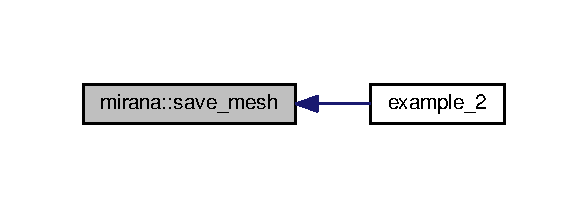
\includegraphics[width=282pt]{classmirana_a9cbee1a318e5e828590c9ccaa51c8472_icgraph}
\end{center}
\end{figure}




The documentation for this module was generated from the following file\-:\begin{DoxyCompactItemize}
\item 
src/\hyperlink{mirana_8f90}{mirana.\-f90}\end{DoxyCompactItemize}

\chapter{File Documentation}
\hypertarget{example__1_8f90}{\section{demo/example\-\_\-1.f90 File Reference}
\label{example__1_8f90}\index{demo/example\-\_\-1.\-f90@{demo/example\-\_\-1.\-f90}}
}
\subsection*{Functions/\-Subroutines}
\begin{DoxyCompactItemize}
\item 
program \hyperlink{example__1_8f90_a33b791e70f7381682d35121a46397153}{example\-\_\-1}
\begin{DoxyCompactList}\small\item\em Test for ordinary differentiation. \end{DoxyCompactList}\end{DoxyCompactItemize}


\subsection{Function/\-Subroutine Documentation}
\hypertarget{example__1_8f90_a33b791e70f7381682d35121a46397153}{\index{example\-\_\-1.\-f90@{example\-\_\-1.\-f90}!example\-\_\-1@{example\-\_\-1}}
\index{example\-\_\-1@{example\-\_\-1}!example_1.f90@{example\-\_\-1.\-f90}}
\subsubsection[{example\-\_\-1}]{\setlength{\rightskip}{0pt plus 5cm}program example\-\_\-1 (
\begin{DoxyParamCaption}
{}
\end{DoxyParamCaption}
)}}\label{example__1_8f90_a33b791e70f7381682d35121a46397153}


Test for ordinary differentiation. 



Here is the call graph for this function\-:\nopagebreak
\begin{figure}[H]
\begin{center}
\leavevmode
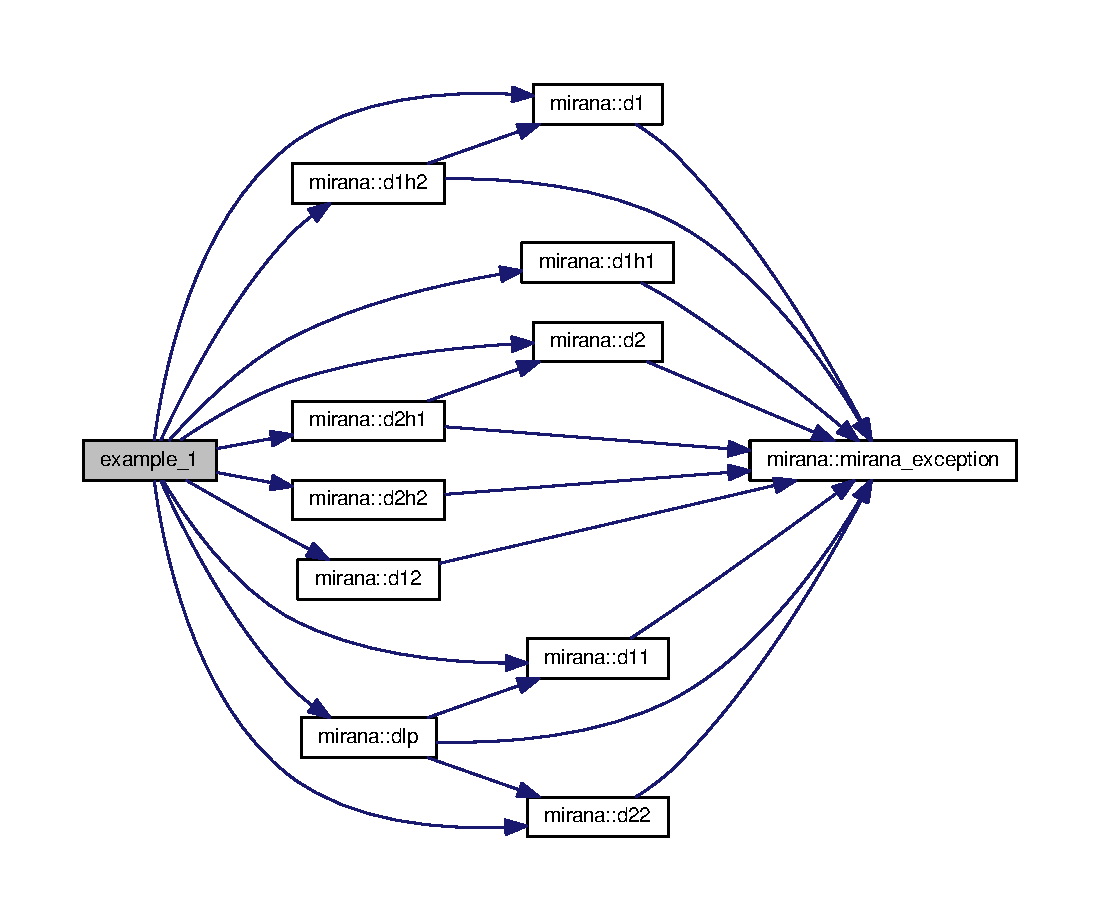
\includegraphics[width=350pt]{example__1_8f90_a33b791e70f7381682d35121a46397153_cgraph}
\end{center}
\end{figure}



\hypertarget{example__2_8f90}{\section{demo/example\-\_\-2.f90 File Reference}
\label{example__2_8f90}\index{demo/example\-\_\-2.\-f90@{demo/example\-\_\-2.\-f90}}
}
\subsection*{Functions/\-Subroutines}
\begin{DoxyCompactItemize}
\item 
program \hyperlink{example__2_8f90_abc1eb48381332994bda2f9fa625923b1}{example\-\_\-2}
\begin{DoxyCompactList}\small\item\em Test for mesh differentiation. \end{DoxyCompactList}\end{DoxyCompactItemize}


\subsection{Function/\-Subroutine Documentation}
\hypertarget{example__2_8f90_abc1eb48381332994bda2f9fa625923b1}{\index{example\-\_\-2.\-f90@{example\-\_\-2.\-f90}!example\-\_\-2@{example\-\_\-2}}
\index{example\-\_\-2@{example\-\_\-2}!example_2.f90@{example\-\_\-2.\-f90}}
\subsubsection[{example\-\_\-2}]{\setlength{\rightskip}{0pt plus 5cm}program example\-\_\-2 (
\begin{DoxyParamCaption}
{}
\end{DoxyParamCaption}
)}}\label{example__2_8f90_abc1eb48381332994bda2f9fa625923b1}


Test for mesh differentiation. 



Here is the call graph for this function\-:\nopagebreak
\begin{figure}[H]
\begin{center}
\leavevmode
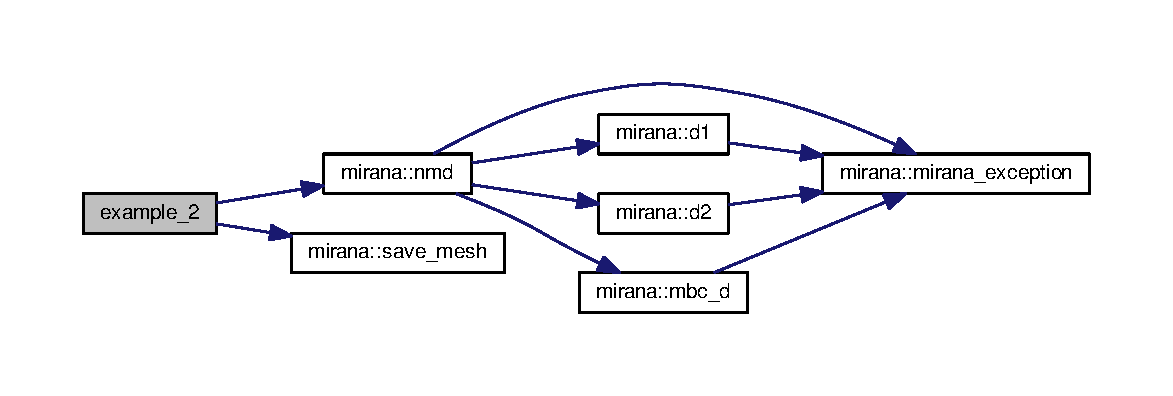
\includegraphics[width=350pt]{example__2_8f90_abc1eb48381332994bda2f9fa625923b1_cgraph}
\end{center}
\end{figure}



\hypertarget{example__3_8f90}{}\section{demo/example\+\_\+3.f90 File Reference}
\label{example__3_8f90}\index{demo/example\+\_\+3.\+f90@{demo/example\+\_\+3.\+f90}}
\subsection*{Functions/\+Subroutines}
\begin{DoxyCompactItemize}
\item 
program \hyperlink{example__3_8f90_a108de56d32a57564c265cb8e2c53a632}{example\+\_\+3}
\begin{DoxyCompactList}\small\item\em Test for differentiation on the moving mesh. \end{DoxyCompactList}\end{DoxyCompactItemize}


\subsection{Function/\+Subroutine Documentation}
\hypertarget{example__3_8f90_a108de56d32a57564c265cb8e2c53a632}{}\index{example\+\_\+3.\+f90@{example\+\_\+3.\+f90}!example\+\_\+3@{example\+\_\+3}}
\index{example\+\_\+3@{example\+\_\+3}!example\+\_\+3.\+f90@{example\+\_\+3.\+f90}}
\subsubsection[{example\+\_\+3}]{\setlength{\rightskip}{0pt plus 5cm}program example\+\_\+3 (
\begin{DoxyParamCaption}
{}
\end{DoxyParamCaption}
)}\label{example__3_8f90_a108de56d32a57564c265cb8e2c53a632}


Test for differentiation on the moving mesh. 



Here is the call graph for this function\+:\nopagebreak
\begin{figure}[H]
\begin{center}
\leavevmode
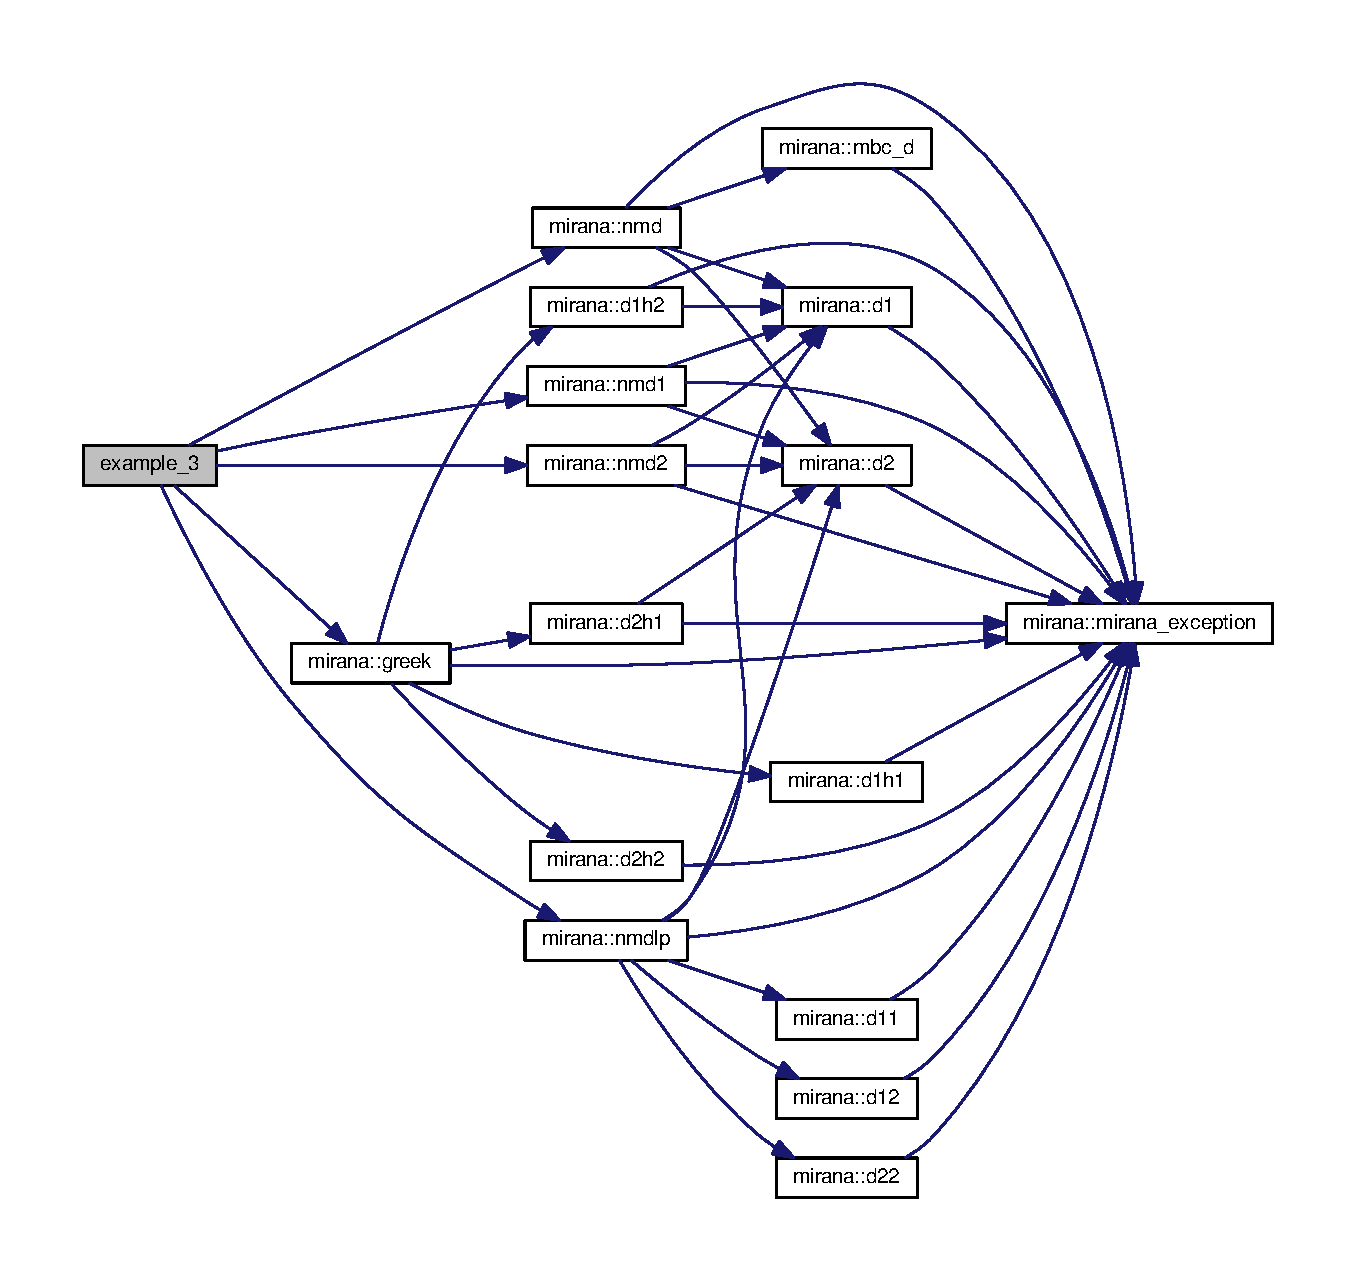
\includegraphics[width=350pt]{example__3_8f90_a108de56d32a57564c265cb8e2c53a632_cgraph}
\end{center}
\end{figure}



\hypertarget{README_8md}{}\section{R\+E\+A\+D\+M\+E.\+md File Reference}
\label{README_8md}\index{R\+E\+A\+D\+M\+E.\+md@{R\+E\+A\+D\+M\+E.\+md}}

\hypertarget{mirana_8f90}{}\section{src/mirana.f90 File Reference}
\label{mirana_8f90}\index{src/mirana.\+f90@{src/mirana.\+f90}}
\subsection*{Modules}
\begin{DoxyCompactItemize}
\item 
module \hyperlink{namespacemirana}{mirana}
\begin{DoxyCompactList}\small\item\em Provide the subroutines \& functions for moving mesh computation. \end{DoxyCompactList}\end{DoxyCompactItemize}
\subsection*{Functions/\+Subroutines}
\begin{DoxyCompactItemize}
\item 
subroutine \hyperlink{namespacemirana_ab002a22665f70b4c65bdcf70ac96d768}{mirana\+::mirana\+\_\+exception} (message)
\begin{DoxyCompactList}\small\item\em Handling exceptions. \end{DoxyCompactList}\item 
subroutine \hyperlink{namespacemirana_acccf612b21e3e65bd3a78131c48afe2b}{mirana\+::mirana\+\_\+memory} (name, dim1, dim2)
\begin{DoxyCompactList}\small\item\em Allocate memory for new arrays. \end{DoxyCompactList}\item 
subroutine \hyperlink{namespacemirana_a9cbee1a318e5e828590c9ccaa51c8472}{mirana\+::save\+\_\+mesh} (mx, my)
\begin{DoxyCompactList}\small\item\em Write mesh data into .dat file for plot. \end{DoxyCompactList}\item 
subroutine \hyperlink{namespacemirana_a4009036e8b04ac992641e36d34ab0ed4}{mirana\+::d1} (phi, h, phi\+\_\+x)
\begin{DoxyCompactList}\small\item\em Differentiate with respect to the first dimension using central difference. \end{DoxyCompactList}\item 
subroutine \hyperlink{namespacemirana_a21348ffe170eafc6fc2a009256b1b6e3}{mirana\+::d2} (phi, h, phi\+\_\+y)
\begin{DoxyCompactList}\small\item\em Differentiate with respect to the second dimension using central difference. \end{DoxyCompactList}\item 
subroutine \hyperlink{namespacemirana_acc84c99770972f6328e89ac04ac67153}{mirana\+::d1h1} (phi, h, phi\+\_\+1h)
\begin{DoxyCompactList}\small\item\em Compute the derivative along the 1st direction at the 1st kind of half points using central difference. \end{DoxyCompactList}\item 
subroutine \hyperlink{namespacemirana_a9d6168761271912ebfea872e9f322cdc}{mirana\+::d1h2} (phi, h, phi\+\_\+1h)
\begin{DoxyCompactList}\small\item\em Compute the derivative along the 1st direction at the 2nd kind of half points using central difference. \end{DoxyCompactList}\item 
subroutine \hyperlink{namespacemirana_a9341f957abd27c5132c557ae873055bd}{mirana\+::d2h1} (phi, h, phi\+\_\+2h)
\begin{DoxyCompactList}\small\item\em Compute the derivative along the 2nd direction at the 1st kind of half points using central difference. \end{DoxyCompactList}\item 
subroutine \hyperlink{namespacemirana_a4f47c93df57dd51d1414b2514fd1b339}{mirana\+::d2h2} (phi, h, phi\+\_\+2h)
\begin{DoxyCompactList}\small\item\em Compute the derivative along the 2nd direction at the 2nd kind of half points using central difference. \end{DoxyCompactList}\item 
subroutine \hyperlink{namespacemirana_ab9b1e7b5e38c6a020e05196b452e6d02}{mirana\+::d11} (phi, h, phi\+\_\+xx)
\begin{DoxyCompactList}\small\item\em Compute the second order derivative along the first dimension using central difference. \end{DoxyCompactList}\item 
subroutine \hyperlink{namespacemirana_ae9ee4058ea2b6238b6b745e4468f6a8e}{mirana\+::d12} (phi, h1, h2, phi\+\_\+xy)
\begin{DoxyCompactList}\small\item\em Comopute the mixed second order derivative using central difference. \end{DoxyCompactList}\item 
subroutine \hyperlink{namespacemirana_a9161b0947ddd188ac99d9246a1d81aed}{mirana\+::d22} (phi, h, phi\+\_\+yy)
\begin{DoxyCompactList}\small\item\em Compute the second order derivative along the second dimension using central difference. \end{DoxyCompactList}\item 
subroutine \hyperlink{namespacemirana_a353bce8a93046cd8fd25021634d6503e}{mirana\+::dlp} (phi, h1, h2, phi\+\_\+lp)
\begin{DoxyCompactList}\small\item\em Compute Laplacian using central difference. \end{DoxyCompactList}\item 
subroutine \hyperlink{namespacemirana_a53c223d4530275ef3fc6a5820f5b0990}{mirana\+::nmd} (mx, my, hxi, het, jcb, xi\+\_\+x, xi\+\_\+y, et\+\_\+x, et\+\_\+y)
\begin{DoxyCompactList}\small\item\em (Non-\/conservative Mesh Differentiation) Compute derivatives of mesh grid with respect to computational space and inverse using non-\/conservative form central difference. \end{DoxyCompactList}\item 
subroutine \hyperlink{namespacemirana_a7530ea2e7b2dfe85f3a088d24de59f1d}{mirana\+::greek} (mx, my, xix, xiy, etx, ety, h1, h2, alp, bet)
\begin{DoxyCompactList}\small\item\em Compute the two coefficients for transformed laplacian $\alpha,\beta$. \end{DoxyCompactList}\item 
subroutine \hyperlink{namespacemirana_a65a514d206d0e8ae53253938d2aff553}{mirana\+::mbc\+\_\+d} (x1, x2, y1, y2)
\begin{DoxyCompactList}\small\item\em (Mesh Boundary Condition for Derivatives) Set the boundary condition of the moving mesh. \end{DoxyCompactList}\end{DoxyCompactItemize}

%--- End generated contents ---

% Index
\newpage
\phantomsection
\addcontentsline{toc}{chapter}{Index}
\printindex

\end{document}
